% Options for packages loaded elsewhere
% Options for packages loaded elsewhere
\PassOptionsToPackage{unicode}{hyperref}
\PassOptionsToPackage{hyphens}{url}
\PassOptionsToPackage{dvipsnames,svgnames,x11names}{xcolor}
%
\documentclass[
  10pt,
  letterpaper,
  DIV=11,
  numbers=noendperiod]{scrartcl}
\usepackage{xcolor}
\usepackage{amsmath,amssymb}
\setcounter{secnumdepth}{5}
\usepackage{iftex}
\ifPDFTeX
  \usepackage[T1]{fontenc}
  \usepackage[utf8]{inputenc}
  \usepackage{textcomp} % provide euro and other symbols
\else % if luatex or xetex
  \usepackage{unicode-math} % this also loads fontspec
  \defaultfontfeatures{Scale=MatchLowercase}
  \defaultfontfeatures[\rmfamily]{Ligatures=TeX,Scale=1}
\fi
\usepackage{lmodern}
\ifPDFTeX\else
  % xetex/luatex font selection
\fi
% Use upquote if available, for straight quotes in verbatim environments
\IfFileExists{upquote.sty}{\usepackage{upquote}}{}
\IfFileExists{microtype.sty}{% use microtype if available
  \usepackage[]{microtype}
  \UseMicrotypeSet[protrusion]{basicmath} % disable protrusion for tt fonts
}{}
% Make \paragraph and \subparagraph free-standing
\makeatletter
\ifx\paragraph\undefined\else
  \let\oldparagraph\paragraph
  \renewcommand{\paragraph}{
    \@ifstar
      \xxxParagraphStar
      \xxxParagraphNoStar
  }
  \newcommand{\xxxParagraphStar}[1]{\oldparagraph*{#1}\mbox{}}
  \newcommand{\xxxParagraphNoStar}[1]{\oldparagraph{#1}\mbox{}}
\fi
\ifx\subparagraph\undefined\else
  \let\oldsubparagraph\subparagraph
  \renewcommand{\subparagraph}{
    \@ifstar
      \xxxSubParagraphStar
      \xxxSubParagraphNoStar
  }
  \newcommand{\xxxSubParagraphStar}[1]{\oldsubparagraph*{#1}\mbox{}}
  \newcommand{\xxxSubParagraphNoStar}[1]{\oldsubparagraph{#1}\mbox{}}
\fi
\makeatother


\usepackage{longtable,booktabs,array}
\usepackage{calc} % for calculating minipage widths
% Correct order of tables after \paragraph or \subparagraph
\usepackage{etoolbox}
\makeatletter
\patchcmd\longtable{\par}{\if@noskipsec\mbox{}\fi\par}{}{}
\makeatother
% Allow footnotes in longtable head/foot
\IfFileExists{footnotehyper.sty}{\usepackage{footnotehyper}}{\usepackage{footnote}}
\makesavenoteenv{longtable}
\usepackage{graphicx}
\makeatletter
\newsavebox\pandoc@box
\newcommand*\pandocbounded[1]{% scales image to fit in text height/width
  \sbox\pandoc@box{#1}%
  \Gscale@div\@tempa{\textheight}{\dimexpr\ht\pandoc@box+\dp\pandoc@box\relax}%
  \Gscale@div\@tempb{\linewidth}{\wd\pandoc@box}%
  \ifdim\@tempb\p@<\@tempa\p@\let\@tempa\@tempb\fi% select the smaller of both
  \ifdim\@tempa\p@<\p@\scalebox{\@tempa}{\usebox\pandoc@box}%
  \else\usebox{\pandoc@box}%
  \fi%
}
% Set default figure placement to htbp
\def\fps@figure{htbp}
\makeatother





\setlength{\emergencystretch}{3em} % prevent overfull lines

\providecommand{\tightlist}{%
  \setlength{\itemsep}{0pt}\setlength{\parskip}{0pt}}



 


\usepackage{xcolor, soul}
\definecolor{Light}{gray}{.90}
\sethlcolor{Light}
\let\OldTexttt\texttt
\renewcommand{\texttt}[1]{\OldTexttt{\hl{#1}}}
\usepackage{caption}
\captionsetup{font=small, labelfont=bf}
\setlength{\parindent}{0pt}
\setlength{\parskip}{1.25ex}
\KOMAoption{captions}{tableheading}
\makeatletter
\@ifpackageloaded{caption}{}{\usepackage{caption}}
\AtBeginDocument{%
\ifdefined\contentsname
  \renewcommand*\contentsname{Table of contents}
\else
  \newcommand\contentsname{Table of contents}
\fi
\ifdefined\listfigurename
  \renewcommand*\listfigurename{List of Figures}
\else
  \newcommand\listfigurename{List of Figures}
\fi
\ifdefined\listtablename
  \renewcommand*\listtablename{List of Tables}
\else
  \newcommand\listtablename{List of Tables}
\fi
\ifdefined\figurename
  \renewcommand*\figurename{Figure}
\else
  \newcommand\figurename{Figure}
\fi
\ifdefined\tablename
  \renewcommand*\tablename{Table}
\else
  \newcommand\tablename{Table}
\fi
}
\@ifpackageloaded{float}{}{\usepackage{float}}
\floatstyle{ruled}
\@ifundefined{c@chapter}{\newfloat{codelisting}{h}{lop}}{\newfloat{codelisting}{h}{lop}[chapter]}
\floatname{codelisting}{Listing}
\newcommand*\listoflistings{\listof{codelisting}{List of Listings}}
\makeatother
\makeatletter
\makeatother
\makeatletter
\@ifpackageloaded{caption}{}{\usepackage{caption}}
\@ifpackageloaded{subcaption}{}{\usepackage{subcaption}}
\makeatother
\usepackage{bookmark}
\IfFileExists{xurl.sty}{\usepackage{xurl}}{} % add URL line breaks if available
\urlstyle{same}
\hypersetup{
  pdftitle={Matched-reliability Mahalanobis distance comparisons},
  pdfauthor={Al Xin},
  colorlinks=true,
  linkcolor={blue},
  filecolor={Maroon},
  citecolor={Blue},
  urlcolor={Blue},
  pdfcreator={LaTeX via pandoc}}


\title{Matched-reliability Mahalanobis distance comparisons}
\author{Al Xin}
\date{Sep 8, 2026}
\begin{document}
\maketitle


\section{Data}\label{data}

\subsection{Stimulus details}\label{stimulus-details}

The stimulus labels are:

\begin{itemize}
\tightlist
\item
  \texttt{coherence}: \texttt{0} when blank, \texttt{1} when noisy,
  \texttt{2} when naturalistic.
\item
  \texttt{family}: \texttt{0} when blank, two or three digit integer
  code otherwise.
\item
  \texttt{id}: \texttt{0} when blank, integer from \texttt{1} to
  \texttt{15} otherwise.
\item
  \texttt{coherence\_t3}: special column for coding coherence in
  \texttt{textures3} (can be ignored)
\item
  \texttt{block\_order}: the relative position of the stimulus in the
  block of 8 image (can be ignored)
\item
  \texttt{repetition}: integer from \texttt{1} to \texttt{100} if blank,
  \texttt{1} to \texttt{6} otherwise.
\end{itemize}

For the final column, when coherence is not zero (non-blank images), the
column contains values 1 through 6 corresponding to the repetition
number.

For blank images, the final column takes on values 1 through 100,
repeating 6 times. Previously, I grouped all blank stimuli together.
However, when prepping data for general use, the blank repetitions need
to be treated more carefully. E.g., permutation testing might require
only permuting within blocked repetitions. For non-blank images, the
\texttt{repetition} label is ordered according to when the images were
presented. For blank images, the rows remain ordered chronologically.

\section{Onset times}\label{onset-times}

The criteria for onset time identification is somewhat strict, requiring
that the \(d'\) between non-blank and blank images exceeds a magnitude
of 0.4 for three consecutive windows (keeping the sign consistent). IT
has the lowest proportion of sites with valid onset times. In general,
onset times seem to get longer with higher visual areas (see
Figure~\ref{fig-onsets_all}).

\begin{figure}

\centering{

\pandocbounded{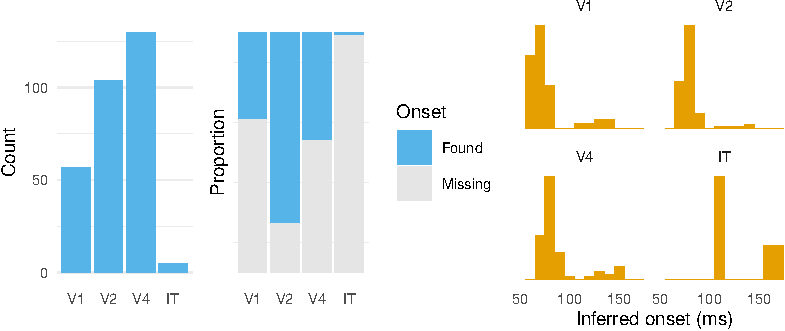
\includegraphics[keepaspectratio]{20260826_files/figure-pdf/fig-onsets_all-1.pdf}}

}

\caption{\label{fig-onsets_all}(Left) The number of sites with a
calculated onset time given the d' criteria, sorted by region. (Center)
The proportion of sites in each region with a calculated onset time. IT
has both the lowest absolute number and lowest proportion of valid onset
times. (Right) Histograms of the calculated onset times per region, with
normalized bar heights.}

\end{figure}%

The effect of onset time calculation (e.g., modifying it to be
calculated only on naturalistic images) is likely a question for another
day.

\section{Pre-computing splits}\label{pre-computing-splits}

There are 20 possible ways to split the 6 repetitions into two groups.
For some analyses, I found it a bit easier to front-load computations
and memory usage and pre-calculate the averages (taken over sample
images) per each of the 20 possible splits.

(This is actually probably not that useful but will be kept in
\texttt{/scratch} in the \texttt{levi2.stat.cmu.edu} server).

\section{Split-half correlation
calculation}\label{split-half-correlation-calculation}

The function \texttt{split\_half\_corr()} in
\texttt{R/responsive\_sites.R} needs a small modification to work with
pre-computed splits. Otherwise, the procedure proceeds as usual.
Split-half correlation calculation can be somewhat stabilized by first
aggregating the observations. Gerrick originally averaged over families
and coherence, but this creates some selection bias for sites that are
responsive at the family level. For our purposes, averaging only over
sample images would be more reasonable.

The observations are first split into two arbitrary groups of 3
repetitions each. The rows are then averaged by the appropriate grouping
(family or sample image) and over a 150 ms window after the temporary
onset time calculated previously. The correlation is then calculated
over the two resulting vectors. For example, for aggregating over sample
images produces two vectors of length 1150 each (1050 sample images +
100 blank images). The blanks can be averaged to produce a vector of
length 1051; I tested approaches with 100 separated blank groups, 1
aggregated blank group, and 0 blank groups (blanks entirely omitted).

I tested correlations over all \(\binom{6}{3} = 20\) splitting
possibilities. The per-site averages are shown as histograms in
Figure~\ref{fig-split_corrs}. The handling of the blank images does not
produce a large difference in the observed correlations, so I will
default to the single aggregated blank group.

See Figure~\ref{fig-corrs_ecdf} for empirical CDFs for the split-half
correlations. Aggregating within family (Gerick's method) or by sample
image (our approach) produces very different distributions. For
within-family aggregation, the split-half correlations tend to be much
higher, with V1, V2, and V4 showing a sharp upturn in the eCDF at around
\(\rho \approx 0.8\).

\begin{figure}

\centering{

\pandocbounded{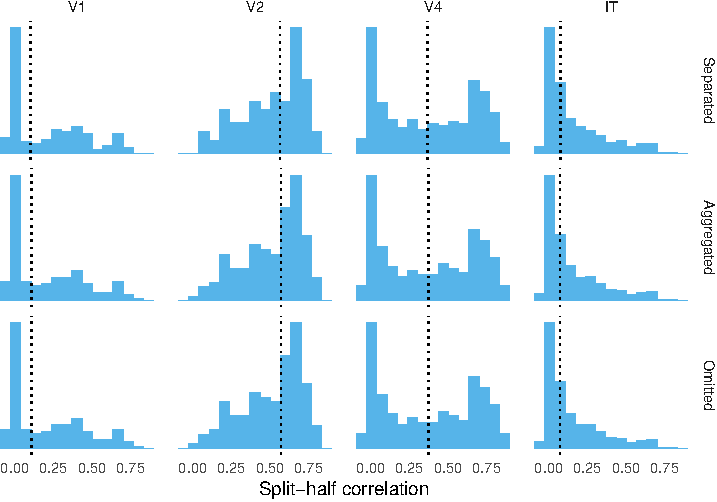
\includegraphics[keepaspectratio]{20260826_files/figure-pdf/fig-split_corrs-1.pdf}}

}

\caption{\label{fig-split_corrs}Normalized histograms of the split-half
correlations calculated for each site, averaged across the 20 possible
splits. The rows indicate the handling of blank images included in the
vectors used for the split-half correlation calculation, with blanks
either omitted entirely, aggregated over all repetitions, or separated
into 100 instances of 6 repetitions each. Dashed lines mark the median.
The distribution of correlations for V1 and IT are more right-shewed.
Differences between the number of blank images are slight, though in
general, the median correlation is lowest when including separated blank
images (with the exception of IT).}

\end{figure}%

\begin{figure}

\centering{

\pandocbounded{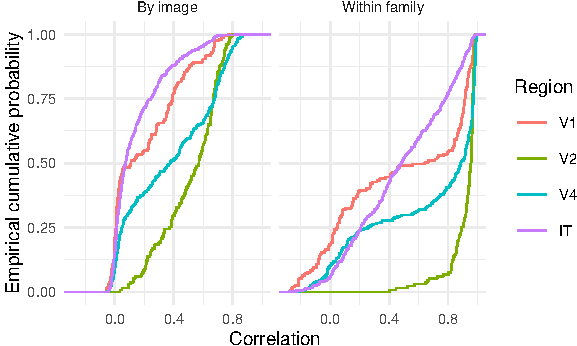
\includegraphics[keepaspectratio]{20260826_files/figure-pdf/fig-corrs_ecdf-1.pdf}}

}

\caption{\label{fig-corrs_ecdf}Empirical cumulative distribution
functions for the split-half correlations by region. Data reflects
split-half correlations performed when all blanks are averaged. (Left)
Aggregated by sample image. (Right) Aggregated by family. For non-IT
regions, the correlations tend to concentrate at above 0.8.}

\end{figure}%

\section{Onset times on reliable
sites}\label{onset-times-on-reliable-sites}

As a reminder, the onsets in Figure~\ref{fig-onsets_all} (which informed
the averaging in Figure~\ref{fig-split_corrs}) were taken over all
sites. We can sanity check if the onset times change based on the
reliable site calculation. Overall, I think it makes sense to retain the
temporary onset times unless there's evidence that it changes a lot
(more than 30 ms).

Taking sites above a split-half correlation of 0.4 or taking sites in
the 80th percentile of correlations doesn't move the onset time much,
though it gets very slightly earlier in V2 for the percentile cutoff.

Thus, I'll use the averages calculated according to the temporary onset
times.

\section{Pairwise between-family Mahalanobis
distance}\label{pairwise-between-family-mahalanobis-distance}

For now, let's take a somewhat arbitrary ``matched-reliability''
criteria of sites with split-half correlation between 0.3 and 0.6. This
yields 39 sites in V1, 49 sites in V2, 57 sites in V4, and 53 sites in
IT. I chose this criteria because the slopes of the lines in
Figure~\ref{fig-corrs_ecdf} look fairly similar within this window.

Figure~\ref{fig-dM_dist} shows the results from a single arbitrary
subsample of 30 sites from each region alongside the split-half
correlations for each site for reference. Figure~\ref{fig-dM_grp}
compares the results with a single subsample when reliable sites are
selected based on the split-half correlations obtained when aggregating
over family. When reliability is calculated after grouping by family,
the distances in IT look like they might be lower than V4, breaking the
trend seen when grouping by image.

However, for family-wise aggregation, it's difficult to find an interval
where the eCDFs of the site split-half correlations are similar between
regions, so the distribution of the split-half correlations used in the
calculations look very skewed for V1, V2, and V4.

\begin{figure}

\centering{

\pandocbounded{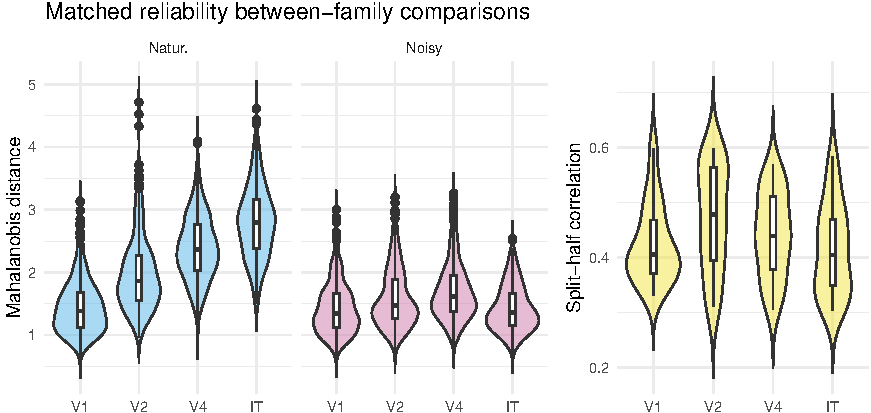
\includegraphics[keepaspectratio]{20260826_files/figure-pdf/fig-dM_dist-1.pdf}}

}

\caption{\label{fig-dM_dist}(Left) Violin plots of the pairwise
between-family Mahalanobis distances, showing a trend of increasing
distance with higher visual areas. The plots for noisy textures are
included for a comparison, showing noisy distances tend to be shorter
with no obvious trend between areas. (Right) The split-half correlations
of the sites included in the left violin plots show differences in
distributions between regions. However, the trends in these
distributions do not seem to be aligned with the trends in the
naturalistic Mahalanobis distances.}

\end{figure}%

\begin{figure}

\centering{

\pandocbounded{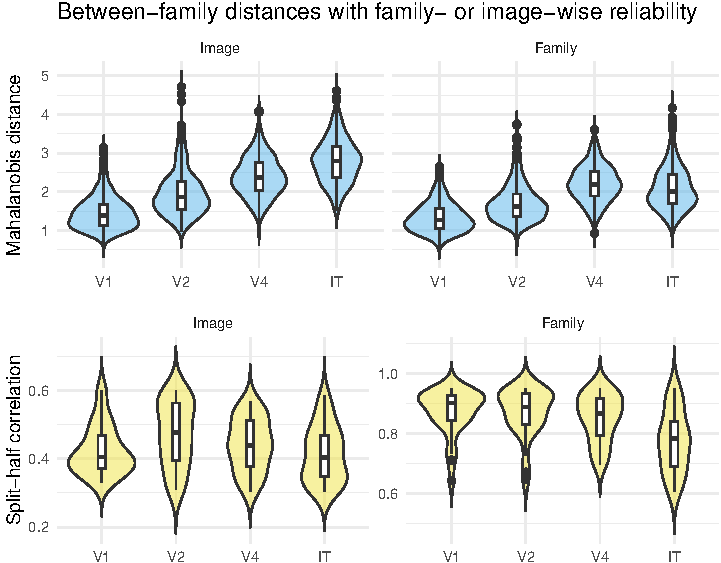
\includegraphics[keepaspectratio]{20260826_files/figure-pdf/fig-dM_grp-1.pdf}}

}

\caption{\label{fig-dM_grp}Comparison of the pairwise between-family
distances when reliable sites are determined by aggregation over
specific sample images (left) or within texture families (right). It is
difficult to match reliability distributions for within-family
aggregation, as correlations in V1, V2, and V4 tend to cluster around
high correlations.}

\end{figure}%

\section{Randomized dichotomies}\label{randomized-dichotomies}

Figure~\ref{fig-rd} is the between-sample analogue to
Figure~\ref{fig-dM_dist}, and shows the results from a single arbitrary
subsample of 30 sites from each region alongside the split-half
correlations for each site for reference. Note that the split-half
correlations are identical to Figure~\ref{fig-dM_dist} sisnce the sites
were generated from the same seed and were not resampled during
randomized dichotomy calculations.

Unlike the between-family comparisons, the Mahalanobis distances look
similar between naturalistic and noisy texture stimuli. This is not
surprising, as the noisy texture stimuli lack any of the higher-order
statistics that would produce a well-defined texture family.

Furthermore, the trends in the split-half correlations seem to be a
reasonable explanation for the differences in the Mahalanobis distances,
with higher correlations associated with larger Mahalanobis distances
(though this is maybe not the case in IT).

\begin{figure}

\centering{

\pandocbounded{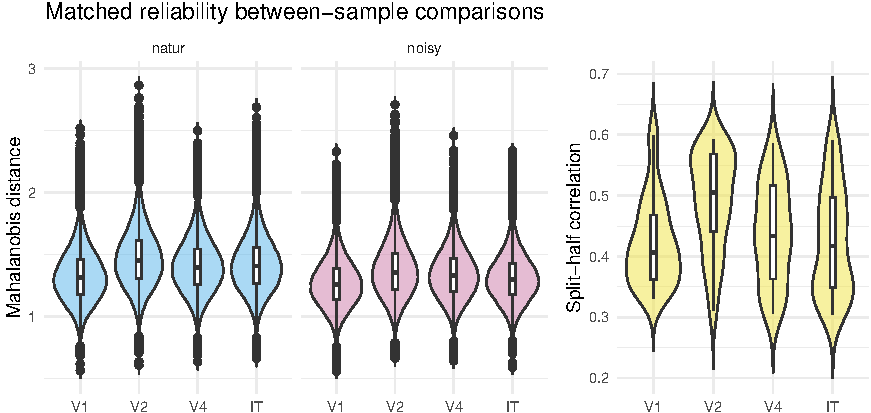
\includegraphics[keepaspectratio]{20260826_files/figure-pdf/fig-rd-1.pdf}}

}

\caption{\label{fig-rd}(Left) Violin plots of the Mahalanobis distances
on randomized dichotomies of sample images, showing roughly equal
distances for all regions. The plots for noisy textures are included for
a comparison, showing naturalistic and noisy distances look comparable.
(Right) The split-half correlations of the sites included in the left
violin plots show differences in distributions between regions. Note
that the distributions are identical to before, as the sites were
subsampled with the same seed. In this case, the mass of the split-half
correlations seems to explain the trend in the randomized dichotomy
distances.}

\end{figure}%




\end{document}
